% ******************************* PhD Thesis Template **************************
% Please have a look at the README.md file for info on how to use the template

\documentclass[a4paper,12pt,times,numbered,print,index]{PhDThesisPSnPDF}

% ******************************************************************************
% ******************************* Class Options ********************************
% *********************** See README for more details **************************
% ******************************************************************************

% `a4paper'(The University of Cambridge PhD thesis guidelines recommends a page
% size a4 - default option) or `a5paper': A5 Paper size is also allowed as per
% the Cambridge University Engineering Deparment guidelines for PhD thesis
%
% `11pt' or `12pt'(default): Font Size 10pt is NOT recommended by the University
% guidelines
%
% `oneside' or `twoside'(default): Printing double side (twoside) or single
% side.
%
% `print': Use `print' for print version with appropriate margins and page
% layout. Leaving the options field blank will activate Online version.
%
% `index': For index at the end of the thesis
%
% `draftclassic': For draft mode without loading any images (same as draft in book)
%
% `draft': Special draft mode with line numbers, images, and water mark with
% timestamp and custom text. Position of the text can also be modified.
%
% `abstract': To generate only the title page and abstract page with
% dissertation title and name, to submit to the Student Registry
%
% `chapter`: This option enables only the specified chapter and its references
%  Useful for review and corrections.
%
% ************************* Custom Page Margins ********************************
%
% `custommargin`: Use `custommargin' in options to activate custom page margins,
% which can be defined in the preamble.tex. Custom margin will override
% print/online margin setup.
%
% *********************** Choosing the Fonts in Class Options ******************
%
% `times' : Times font with math support. (The Cambridge University guidelines
% recommend using times)
%
% `fourier': Utopia Font with Fourier Math font (Font has to be installed)
%            It's a free font.
%
% `customfont': Use `customfont' option in the document class and load the
% package in the preamble.tex
%
% default or leave empty: `Latin Modern' font will be loaded.
%
% ********************** Choosing the Bibliography style ***********************
%
% `authoryear': For author-year citation eg., Krishna (2013)
%
% `numbered': (Default Option) For numbered and sorted citation e.g., [1,5,2]
%
% `custombib': Define your own bibliography style in the `preamble.tex' file.
%              `\RequirePackage[square, sort, numbers, authoryear]{natbib}'.
%              This can be also used to load biblatex instead of natbib
%              (See Preamble)
%
% **************************** Choosing the Page Style *************************
%
% `default (leave empty)': For Page Numbers in Header (Left Even, Right Odd) and
% Chapter Name in Header (Right Even) and Section Name (Left Odd). Blank Footer.
%
% `PageStyleI': Chapter Name next & Page Number on Even Side (Left Even).
% Section Name & Page Number in Header on Odd Side (Right Odd). Footer is empty.
%
% `PageStyleII': Chapter Name on Even Side (Left Even) in Header. Section Number
% and Section Name in Header on Odd Side (Right Odd). Page numbering in footer

% Uncomment to change page style
%\pagestyle{PageStyleII}

% ********************************** Preamble **********************************
% Preamble: Contains packages and user-defined commands and settings
% ******************************************************************************
% ****************************** Custom Margin *********************************

% Add `custommargin' in the document class options to use this section
% Set {innerside margin / outerside margin / topmargin / bottom margin}  and
% other page dimensions
\ifsetCustomMargin
  \RequirePackage[left=37mm,right=30mm,top=35mm,bottom=30mm]{geometry}
  \setFancyHdr % To apply fancy header after geometry package is loaded
\fi

% Add spaces between paragraphs
%\setlength{\parskip}{0.5em}
% Ragged bottom avoids extra whitespaces between paragraphs
\raggedbottom
% To remove the excess top spacing for enumeration, list and description
%\usepackage{enumitem}
%\setlist[enumerate,itemize,description]{topsep=0em}

% *****************************************************************************
% ******************* Fonts (like different typewriter fonts etc.)*************

% Add `customfont' in the document class option to use this section

\ifsetCustomFont
  % Set your custom font here and use `customfont' in options. Leave empty to
  % load computer modern font (default LaTeX font).
  %\RequirePackage{helvet}

  % For use with XeLaTeX
  %  \setmainfont[
  %    Path              = ./libertine/opentype/,
  %    Extension         = .otf,
  %    UprightFont = LinLibertine_R,
  %    BoldFont = LinLibertine_RZ, % Linux Libertine O Regular Semibold
  %    ItalicFont = LinLibertine_RI,
  %    BoldItalicFont = LinLibertine_RZI, % Linux Libertine O Regular Semibold Italic
  %  ]
  %  {libertine}
  %  % load font from system font
  %  \newfontfamily\libertinesystemfont{Linux Libertine O}
\fi

% *****************************************************************************
% **************************** Custom Packages ********************************

% ************************* Algorithms and Pseudocode **************************

%\usepackage{algpseudocode}


% ********************Captions and Hyperreferencing / URL **********************

% Captions: This makes captions of figures use a boldfaced small font.
%\RequirePackage[small,bf]{caption}

\RequirePackage[labelsep=space,tableposition=top]{caption}
\renewcommand{\figurename}{Fig.} %to support older versions of captions.sty


% *************************** Graphics and figures *****************************

%\usepackage{rotating}
%\usepackage{wrapfig}

% Uncomment the following two lines to force Latex to place the figure.
% Use [H] when including graphics. Note 'H' instead of 'h'
%\usepackage{float}
%\restylefloat{figure}

% Subcaption package is also available in the sty folder you can use that by
% uncommenting the following line
% This is for people stuck with older versions of texlive
%\usepackage{sty/caption/subcaption}
\usepackage{subcaption}

% ********************************** Tables ************************************
\usepackage{booktabs} % For professional looking tables
\usepackage{multirow}

%\usepackage{multicol}
%\usepackage{longtable}
%\usepackage{tabularx}


% *********************************** SI Units *********************************
\usepackage{siunitx} % use this package module for SI units


% ******************************* Line Spacing *********************************

% Choose linespacing as appropriate. Default is one-half line spacing as per the
% University guidelines

% \doublespacing
% \onehalfspacing
% \singlespacing


% ************************ Formatting / Footnote *******************************

% Don't break enumeration (etc.) across pages in an ugly manner (default 10000)
%\clubpenalty=500
%\widowpenalty=500

%\usepackage[perpage]{footmisc} %Range of footnote options


% *****************************************************************************
% *************************** Bibliography  and References ********************

%\usepackage{cleveref} %Referencing without need to explicitly state fig /table

% Add `custombib' in the document class option to use this section
\ifuseCustomBib
  \RequirePackage[square, sort, numbers, authoryear]{natbib} % CustomBib

  % If you would like to use biblatex for your reference management, as opposed to the default `natbibpackage` pass the option `custombib` in the document class. Comment out the previous line to make sure you don't load the natbib package. Uncomment the following lines and specify the location of references.bib file

  %\RequirePackage[backend=biber, style=numeric-comp, citestyle=numeric, sorting=nty, natbib=true]{biblatex}
  %\addbibresource{References/references} %Location of references.bib only for biblatex, Do not omit the .bib extension from the filename.

\fi

% changes the default name `Bibliography` -> `References'
\renewcommand{\bibname}{References}


% ******************************************************************************
% ************************* User Defined Commands ******************************
% ******************************************************************************

% *********** To change the name of Table of Contents / LOF and LOT ************

%\renewcommand{\contentsname}{My Table of Contents}
%\renewcommand{\listfigurename}{My List of Figures}
%\renewcommand{\listtablename}{My List of Tables}


% ********************** TOC depth and numbering depth *************************

\setcounter{secnumdepth}{2}
\setcounter{tocdepth}{2}


% ******************************* Nomenclature *********************************

% To change the name of the Nomenclature section, uncomment the following line

%\renewcommand{\nomname}{Symbols}


% ********************************* Appendix ***********************************

% The default value of both \appendixtocname and \appendixpagename is `Appendices'. These names can all be changed via:

%\renewcommand{\appendixtocname}{List of appendices}
%\renewcommand{\appendixname}{Appndx}

% *********************** Configure Draft Mode **********************************

% Uncomment to disable figures in `draft'
%\setkeys{Gin}{draft=true}  % set draft to false to enable figures in `draft'

% These options are active only during the draft mode
% Default text is "Draft"
%\SetDraftText{DRAFT}

% Default Watermark location is top. Location (top/bottom)
%\SetDraftWMPosition{bottom}

% Draft Version - default is v1.0
%\SetDraftVersion{v1.1}

% Draft Text grayscale value (should be between 0-black and 1-white)
% Default value is 0.75
%\SetDraftGrayScale{0.8}


% ******************************** Todo Notes **********************************
%% Uncomment the following lines to have todonotes.

\ifsetDraft
  \usepackage[colorinlistoftodos]{todonotes}
  \newcommand{\mynote}[1]{\todo[author=kks32,size=\small,inline,color=green!40]{#1}}
\else
  \newcommand{\mynote}[1]{}
  \newcommand{\listoftodos}{}
\fi

% Example todo: \mynote{Hey! I have a note}

% ******************************** Highlighting Changes **********************************
%% Uncomment the following lines to be able to highlight text/modifications.
%\ifsetDraft
%  \usepackage{color, soul}
%  \newcommand{\hlc}[2][yellow]{{\sethlcolor{#1} \hl{#2}}}
%  \newcommand{\hlfix}[2]{\texthl{#1}\todo{#2}}
%\else
%  \newcommand{\hlc}[2]{}
%  \newcommand{\hlfix}[2]{}
%\fi

% Example highlight 1: \hlc{Text to be highlighted}
% Example highlight 2: \hlc[green]{Text to be highlighted in green colour}
% Example highlight 3: \hlfix{Original Text}{Fixed Text}

% *****************************************************************************
% ******************* Better enumeration my MB*************
\usepackage{enumitem}


% ************************ Thesis Information & Meta-data **********************
% Thesis title and author information, refernce file for biblatex
% ************************ Thesis Information & Meta-data **********************
%% The title of the thesis
\title{Privacy Preserving Data Access in Edge Computing}
%\texorpdfstring is used for PDF metadata. Usage:
%\texorpdfstring{LaTeX_Version}{PDF Version (non-latex)} eg.,
%\texorpdfstring{$sigma$}{sigma}

%% Subtitle (Optional)
% \subtitle{Using the CUED template}

%% The full name of the author
\author{Ujjwal Goel}

%% Department (eg. Department of Engineering, Maths, Physics)
\dept{Department of Computer Science and Engineering}

%% University and Crest
\university{Indian Institute of Information Technology, Guwahati}
% Crest minimum should be 30mm.
% \crest{\includegraphics[width=0.2\textwidth]{University_Crest}}
%% Use this crest, if you are using the college crest
%% Crest long miminum should be 65mm
%\crest{\includegraphics[width=0.45\textwidth]{University_Crest_Long}}

%% College shield [optional] 
% Crest minimum should be 30mm.
%\collegeshield{\includegraphics[width=0.2\textwidth]{CollegeShields/Kings}}


%% Supervisor (optional)
%% for multiple supervisors, append each supervisor with the \newline command
%\supervisor{Prof. A.B. Supervisor\newline
%Prof. C.D. Supervisor}

%% Supervisor Role (optional) - Supervisor (default) or advisor
% \supervisorrole{\textbf{Supervisors: }}
%% if no title is desired:
% \supervisorrole{}

%% Supervisor line width: required to align supervisors
%\supervisorlinewidth{0.35\textwidth}

%% Advisor (optional)
%% for multiple advisors, append each advisor with the \newline command
\advisor{ \textbf{ Dr. Ferdous Ahmed Barbhuiya } }

%% Advisor Role (optional) - Advisor (default) or leave empty
% \advisorrole{Advisors: }
%% if no title is required
% \advisorrole{}

%% Advisor line width: required to align supervisors
%\advisorlinewidth{0.25\textwidth}


%% You can redefine the submission text:
% Default as per the University guidelines:
% ``This dissertation is submitted for the degree of''
\renewcommand{\submissiontext}{}

%% Full title of the Degree
% \degreetitle{Doctor of Philosophy}

%% College affiliation (optional)
% \college{King's College}

%% Submission date
% Default is set as {\monthname[\the\month]\space\the\year}
%\degreedate{September 2014} 

%% Meta information
\subject{Edge computing} \keywords{{privacy} {data access}}


% ***************************** Abstract Separate ******************************
% To printout only the titlepage and the abstract with the PhD title and the
% author name for submission to the Student Registry, use the `abstract' option in
% the document class.

\ifdefineAbstract
 \pagestyle{empty}
 \includeonly{Declaration/declaration, Abstract/abstract}
\fi

% ***************************** Chapter Mode ***********************************
% The chapter mode allows user to only print particular chapters with references
% Title, Contents, Frontmatter are disabled by default
% Useful option to review a particular chapter or to send it to supervisior.
% To use choose `chapter' option in the document class

\ifdefineChapter
 \includeonly{Chapter3/chapter3}
\fi

% ******************************** Front Matter ********************************
\begin{document}

\frontmatter

\maketitle

\include{Dedication/dedication}
% ******************************* Thesis Declaration ***************************

\begin{declaration}

I hereby declare that except where specific reference is made to the work of 
others, the contents of this dissertation are original and have not been 
submitted in whole or in part for consideration for any other degree or 
qualification in this, or any other university. This dissertation is my own 
work and contains nothing which is the outcome of work done in collaboration 
with others, except as specified in the text and Acknowledgements.

% Author and date will be inserted automatically from thesis.tex \author \degreedate

\end{declaration}


% ************************** Thesis Acknowledgements **************************

\begin{acknowledgements}
    I would like to acknowledge my supervisor, Dr. Ferdous for his constant
    guidance and support throughout the project.

    I would also like to thank Dr. Rakesh Matam, Meghali Nandi, Membub Alam and
    Aditya Sharma for their help and guidance.
\end{acknowledgements}

% ************************** Thesis Abstract ***********************************
% Use `abstract' as an option in the document class to print only the titlepage
% and the abstract.
\begin{abstract}
    In our project, we are working on the problem of secure data access in the
    edge computing environment.
\end{abstract}


% *********************** Adding TOC and List of Figures ***********************

\tableofcontents

\listoffigures

\listoftables

% \printnomenclature[space] space can be set as 2em between symbol and description
%\printnomenclature[3em]

\printnomenclature

% ******************************** Main Matter *********************************
\mainmatter

%!TEX root = ../thesis.tex

\chapter{Introduction}

\graphicspath{{Figs}}

\section{Edge computing}

Edge computing is a newer computation paradigm as compared to cloud computing.
Difference between them is that edge computing begins computation closer to the
edge of the network. As more of the data is being generated near the edge of the
network, edge computing enables the data to be processed near the data source.
\cite{weisongshiEdgeComputingVision2016}

\subsection{Why use edge computing in place of cloud computing?}

The most important reason for using edge computing is that it reduces the
latency as the data has to travel a shorter distance.
\cite{weisongshiEdgeComputingVision2016} In addition to this, with emergence of
Internet of Things, the data generated at the edge is expected to grow rapidly.
For example, it is expected that the autonomous vehicles will generate data in
the order of 1Tb per second. In such a case, it may not be possible for the
cloud to keep pace with the data generated at the edge. Edge computing can help
in this situation as it can process the data at the edge itself.

\subsection{Challenges with edge computing}

One of the major challenges with edge computing is that the edge devices are
resource constrained. They have limited processing power, memory and storage.
Often, this problem is solving using offloading. A node that is low on resources
may enlist the other nodes for help. For example, if a node is low on storage
space, then the data generate on this node or the data this node was supported
to store may be offloaded to other nodes in the network. Similarly, data
processing can be offloaded to other nodes.

Other challenge is that, no node in the edge network has complete knowledge of
the edge network. This is in contrast with cloud computing where a central is
responsible for all the processing and does not need to coordinator with others.
As such, it can become difficult to do any computation on the edge as the nodes
may not be having all the information required for the computation.

\subsection{Edge computing for vehicles}

Researchers have been working on using edge computing for vehicles for a while
now. In autonomous vehicles, the decision must be taken quickly as there is very
low tolerance for latency. Further, the data that a vehicle generate is rarely
needed outside the geographical vicinity in which the vehicle is present. Using
edge computing makes the common use-case faster. As such, edge computing can be
used to improve the performance of the autonomous vehicles.

\begin{figure}[h]
      \centering
      \includegraphics[width=1.0\textwidth]{"Vehicular Edge Network.png"}
      \caption{Vehicular edge network architecture}
\end{figure}

Vehicular edge networks usually consists of a central cloud to which a number of
gateway devices called roadside units (RSUs) are connected. The RSUs are further
connected to the vehicles. Vehicular edge networks are highly dynamic and
vehicles change their position quite often. Because of this, hand-offs may be
needed very frequently.

\section{Problem statement}

Because of the issues described above, we need to have some kind of method to
enable nodes to find out where the required data may be present in the edge
network.

We are trying to come up with a method for answering resource queries in edge
networks while keeping in mind the constraints on resources that come with edge
computing.

Requirements for the solution:
\begin{itemize}
      \item Data privacy is maintained and the data itself should not be used
            for indexing or querying
      \item The solution should be scalable
      \item The algorithm should preferably be online -- it should be able to
            index or answer queries for the data that is being generated
\end{itemize}

Further, it is not possible to simply boardcast the query to all the nodes in
network as it would very inefficient. Doing so will lead to privacy issues as
the queries would be known to every node in the network. Also, caching the data
on other nodes should be avoided because of the privacy issues.

\subsubsection{Use cases}

The problem of resource or data discovery is by no mean unique to edge computing
or IoT. Even in the computer architecture, Flat Cache-Only Memory Architecture
(COMA) faces the similar problem. In Flat COMA, memory lines can freely migrate.
Whenever there is cache miss, the memory line must be located in the network and
migrated to where it is needed.
\cite{joseptorrellasCacheOnlyMemoryArchitecture}

But in our work, we are trying to solve this problem in context of edge
computing where the nodes may be static or dynamic. Weather crowd-sensing would
need only static nodes, but in vehicular edge networks, the nodes are dynamic.


\chapter{Literature review}

Numerous surveys have been done on edge computing as well as data access in IoT
or distributed systems. These include \citet{kouahlaSurveyBigIoT2022} and
\citet{fathyLargeScaleIndexingDiscovery2018}.

\citet{fathyLargeScaleIndexingDiscovery2018} prescribes the following taxonomy
for queries in IoT:

\begin{itemize}
      \item \textbf{Data queries}: Here, we are only interested in the data,
            regardless of its source. The may be indexed by:
            \begin{itemize}
                  \item Spatial features: The data may be indexed using spatial
                        attributes, e.g. geo-coordinates. Space filling curves
                        may be used to reduce dimensionality.
                  \item Thematic features: data is indexed based on the keywords
                        or its attributes.
                  \item Temporal features: data is indexed based on the time at
                        which it was generated.
            \end{itemize}

      \item \textbf{Resource queries}: Rather than finding the data stored on
            the node, the nodes are only interested in finding a physical
            resource on the network.
      \item \textbf{Higher-level abstractions}: the queries are based on
            higher-level abstractions like events, activities and patterns which
            require data from several nodes to be combined and processed.
\end{itemize}

\citet{kouahlaSurveyBigIoT2022} also classifies indexing techniques as below:

\begin{itemize}
      \item Indexing structures in a Multidimensional Space
            \begin{itemize}
                  \item Hashing-based techniques
                  \item Tree-based techniques
                  \item Bitmap-based techniques
            \end{itemize}
      \item Indexing structures in a Metric Space
            \begin{itemize}
                  \item Tree-based techniques
            \end{itemize}
\end{itemize}

In this work, our focus is on resource queries. The advantage of focusing on
resource queries over data queries is that the data queries can be trivially
answered once the resource queries are answered. Further, it allows the nodes to
implement some kind of authentication mechanism to ensure that the data is not
publically available.


In 2012, \citet{federicapaganelliDHTBasedDiscoveryService2012} proposed a scheme
that DHTs for service discovery in Internet of Things. Their method allowed
multi-attribute queries as well as range queries. The method consists of three
layers. They first used a space-filling curve to linearize and map the
multidimensional domain into a one-dimensional one. Then a Prefix-Hash Table is
used on top of a generic DHT with standard interface for get and put. At the
end, the DHT is implementation based on the Kademlia algorithm.
\citet{federicapaganelliDHTBasedDiscoveryService2012}, however, did not apply
DHTs to edge networks.

Researchers have also attempted to use Gaussian Mixture Models (GMM) for
searching and indexing in edge computing.


\section{Distributed Hash Tables}

The Distributed Hash Tables (DHTs) are similar to the conventional hash tables,
except that the key-value pairs are stored across multiple nodes in the network.
Distributed hash tables are highly scalable and fault-tolerant. Like traditional
hash-tables, DHTs also support ``get'' and ``put'' operations. They are commonly
used in the peer-to-peer networks. There exist multiple variants of DHTs
including Chord \cite{ChordScalablePeertopeer}, Tapestry
\cite{zhaoTapestryResilientGlobalscale2004} and Kademlia
\cite{petarmaymounkovKademliaPeertoPeerInformation2002}.

In DHTs, the data is placed deterministically on the nodes in the network. DHTs
are self-organizing and self-healing.

Of these DHTs, Kademlia is the most widely used. It is used in BitTorrent
\cite{andrewloewensternDHTProtocol2008} as well as in Ethereum. Every key-value
pair is stored with multiple nodes in the network. This is done to ensure that
the network is robust to node failures. Kademlia is not affected if a node
leaves or joins the network. Each node joining the Kademlia randomly generates a
160-bit identifier.
\cite{petarmaymounkovKademliaPeertoPeerInformation2002}

\subsection{How Kademlia works?}

Whenever a key-value pair is to be stored in the network, a 160 bit hash of the
key is calculated. Then, nodes with the identifier closest to the hash are
selected for storing the key-value pair. For measuring the distance and finding
the closest nodes to a given key, Kademlia uses XOR metric even though it is
non-euclidean. The XOR metric satisfies all four properties of a distance
metric.
\cite{MetricSpace2022}

Similarly, when finding the value for a given key, the nodes with the identifier
closest to the hash of the key are selected. An attempt is then made to retrieve
the corresponding values from these nodes.

The authors also propose an XOR based routing algorithm for finding the node
with the identifier closest to a given key. With the algorithm proposed, in each
iteration, we get one bit closer to the target node. Thus, if the network size
if $n$, then the algorithm takes $O(log(n))$ iterations to find the target node.

Nodes in Kademlia can visualize as leaves in a binary tree where the position of
each of the nodes is given by its identifier. In the algorithm, each node is
required to maintain a routing table. Each of the node is expected to store
information about $k$ nodes from each of the maximal tree in the that it is not
a part in its routing table. The information includes the identifier, IP address
and the port number. The requirement of storing information about $k$ nodes from
each is to bring redundancy and to ensure that the network is robust to node
failures.

\begin{figure}[h]
      \centering
      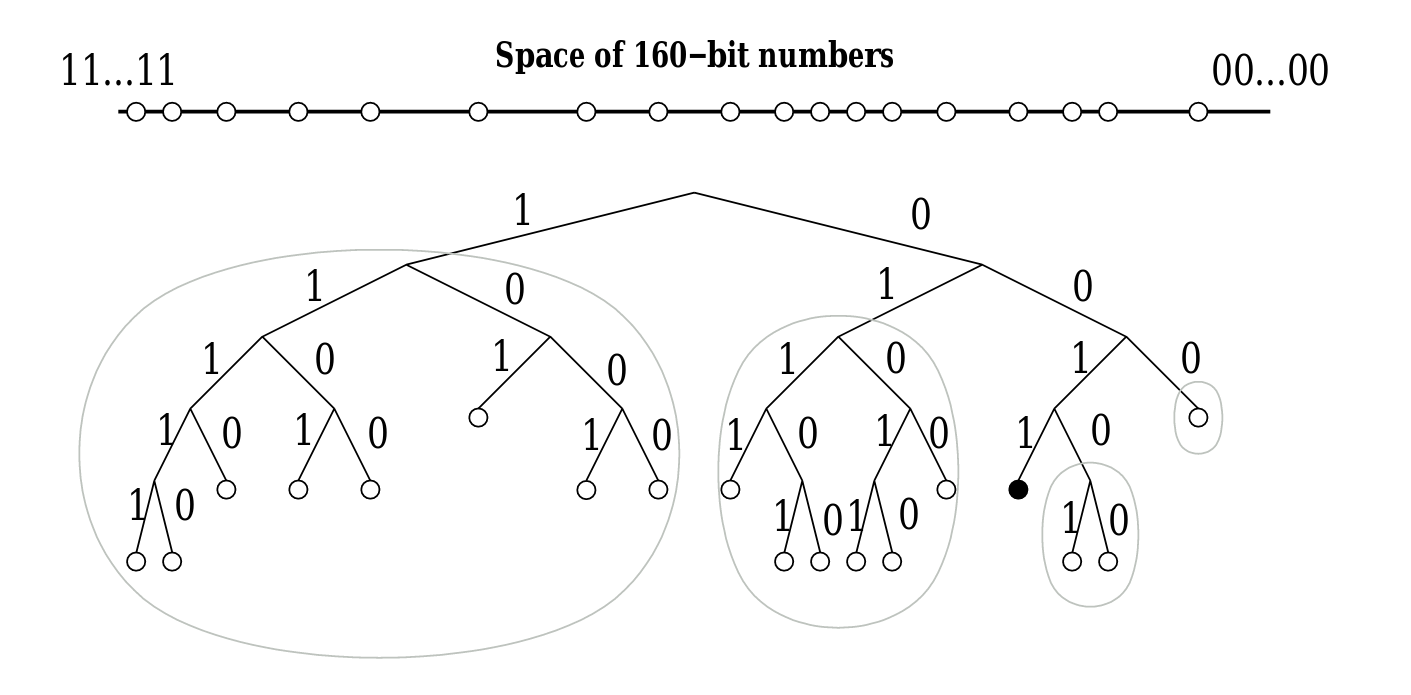
\includegraphics[width=1.0\textwidth]{kademlia.png}
      \caption[Kademlia]{The node with identifier 0011 stores information about
            nodes in four subtrees which are encircled.
            \cite{petarmaymounkovKademliaPeertoPeerInformation2002}}
      % \caption[Routing in Kademlia]
\end{figure}

\section{Learned indexes}

\citet{kraska2018} proposed that machine learning models may be used along with
traditional data structures to improve performance. For example, in a sorted
array, instead of using binary search or an index, a machine learning model may
be used to predict the appropriate index of the element. This can be applied to
many structures like B-trees, bloom filters, etc.

Several learned indexes have been proposed -- Learned Spatial Index
\cite{pandeyCaseLearnedSpatial2020} for answering spatial range queries, Learned
Secondary Index \cite{kipfLSILearnedSecondary2022} for unsorted data,
RadixSpline \cite{kipfRadixSplineSinglePassLearned2020}, an index that can be
built in a single pass and Practical Learned Index (PLEX)
\cite{stoianPracticalLearnedIndexing2021} which was introduced to make the
learned index more practical by reducing the number of hyperparameters to just
one.

Learned indices have recently been gaining popularity in the database community
recently. The idea of using machine learning models has been so influential that
researchers are applying the same approach to even the sorting algorithms.
\cite{kristoCaseLearnedSorting2020}

\citet{kraska2018} also proposed a Recursive Model Index which is hierarchical
in nature. They are similar to B-trees except, a machine learning model is used
in each stage. In each stage, the model predicts another model until the leaf
node is reached where the data is stored. It can also be viewed as each node
picking a better expert to answer the query.

\begin{figure}[h]
      \centering
      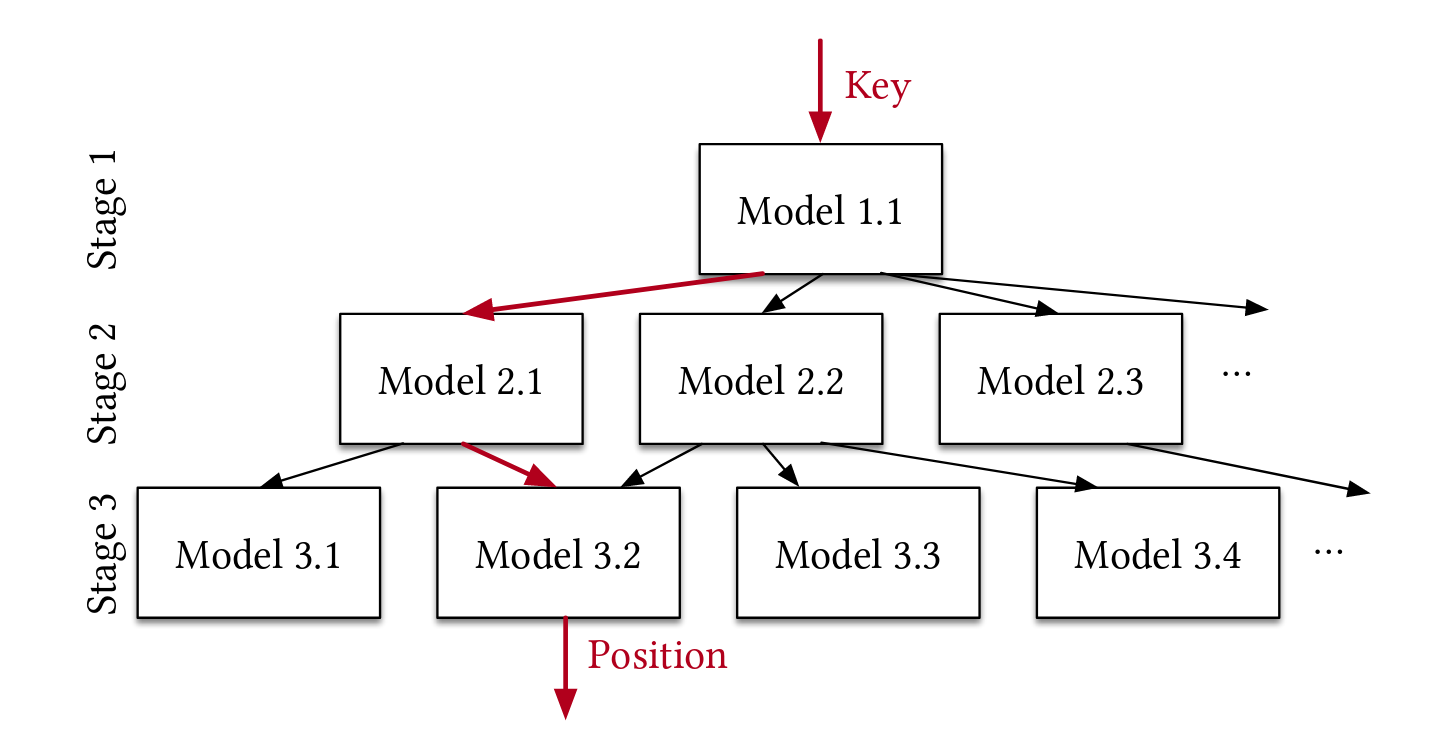
\includegraphics[width=1.0\textwidth]{RMI.png}
      \caption[Recursive Model Index]{The Recursive Model Index.
            \cite{kraska2018}}
\end{figure}
\chapter{Proposed Methodology}

\section{Using Distributed Hash Tables for Edge Computing}

We tried to extend DHTs and learned indices to edge networks. We intend to use
Kademlia not for content discovery, but only the XOR based routing algorithm
proposed by \citet{petarmaymounkovKademliaPeertoPeerInformation2002} for
routing, once the target node is determined using the learned index.

\citet{xieEfficientIndexingMechanism2019} observed that DHTs may use a longer
path than the shortest possible path between two nodes. This happens because the
nodes which may be logically close to each as determined by XOR metric on node
identifier may, in fact, be far apart physically. One possible way of solving
this problem is to modify the node identifier used by Kademlia so that it is
based on the location of the node. \citet{mengweiImprovementKademliaBased2013}
did this by using the IP address of the nodes as the prefix in the node
identifier. While this should make the routing in Kademlia more efficient, this
method suffers from the drawback that the IP address of the node may change.

The another way in which node identifiers can be modified is to encode the
services offered a node into its identifier. For example, if a node is offering
weather sensing service, its identifier may be prefixed by ``10'' or if it is
offering road-traffic information, its identifier may be prefixed by ``01''.
Similarly, if both the services are offered by the node, its identifier may
start with ``11''. Because of how routing works in Kademlia, it would be trivial
to search for nodes offering a particular service if this scheme is used. While
we could not find any work that has done this, we believe that this too will
have limitations.

We used the open-source Python library for testing if Kademlia would be
appropriate for this use case. \cite{KademliaIndexRst}

\section{Using Learned Indices for Edge Computing}


While \citet{kraska2018} proposed that model should be trained only once, but we
believe it would be better if the model is updated periodically so that it can
serve the queries better.

To test the performance of learned indexes, we simulated an edge network using
Python. Inside each edge node, we put five key value pairs. The keys were
randomly generated strings and the values were randomly generated integers.
First, keys were encoded using ordinal encoding. Then a one-vs-rest multi-class
classifier was used to predict the location which the key-value pairs might be
stored. Though the results were not conclusive, using a real world dataset by
\citet{taxi&limousinecommissionNewYorkTaxi} should give conclusive results. This
is because random data carrier the most amount of entropy, it is the most
difficult to compress, and real world data usually has a lot of redundancy and
patterns which the model can learn.

\section{Conclusion}

We believe learned indexes can be a good fit for this problem. Along with
learned indexes, the routing algorithm proposed in Kademlia can be used to
routing after modifying it so that it favors the shortest path between the nodes
based on the scheme proposed by \citet{mengweiImprovementKademliaBased2013}.
% %!TEX root = ../thesis.tex
%*******************************************************************************
%****************************** Second Chapter *********************************
%*******************************************************************************

\chapter{My second chapter}

\graphicspath{{Chapter2/Figs/Raster/}{Chapter2/Figs/PDF/}{Chapter2/Figs/}}


\section[Short title]{Reasonably long section title}

% Uncomment this line, when you have siunitx package loaded.
%The SI Units for dynamic viscosity is \si{\newton\second\per\metre\squared}.
I'm going to randomly include a picture Figure~\ref{fig:minion}.


If you have trouble viewing this document contact Krishna at: \href{mailto:kks32@cam.ac.uk}{kks32@cam.ac.uk} or raise an issue at \url{https://github.com/kks32/phd-thesis-template/}


\begin{figure}[htbp!] 
\centering    
\includegraphics[width=1.0\textwidth]{minion.png}
\caption[Minion]{This is just a long figure caption for the minion in Despicable Me from Pixar}
\label{fig:minion}
\end{figure}


\section*{Enumeration}
Lorem ipsum dolor sit amet, consectetur adipiscing elit. Sed vitae laoreet lectus. Donec lacus quam, malesuada ut erat vel, consectetur eleifend tellus. Aliquam non feugiat lacus. Interdum et malesuada fames ac ante ipsum primis in faucibus. Quisque a dolor sit amet dui malesuada malesuada id ac metus. Phasellus posuere egestas mauris, sed porta arcu vulputate ut. Donec arcu erat, ultrices et nisl ut, ultricies facilisis urna. Quisque iaculis, lorem non maximus pretium, dui eros auctor quam, sed sodales libero felis vel orci. Aliquam neque nunc, elementum id accumsan eu, varius eu enim. Aliquam blandit ante et ligula tempor pharetra. Donec molestie porttitor commodo. Integer rutrum turpis ac erat tristique cursus. Sed venenatis urna vel tempus venenatis. Nam eu rhoncus eros, et condimentum elit. Quisque risus turpis, aliquam eget euismod id, gravida in odio. Nunc elementum nibh risus, ut faucibus mauris molestie eu.
 Vivamus quis nunc nec nisl vulputate fringilla. Duis tempus libero ac justo laoreet tincidunt. Fusce sagittis gravida magna, pharetra venenatis mauris semper at. Nullam eleifend felis a elementum sagittis. In vel turpis eu metus euismod tempus eget sit amet tortor. Donec eu rhoncus libero, quis iaculis lectus. Aliquam erat volutpat. Proin id ullamcorper tortor. Fusce vestibulum a enim non volutpat. Nam ut interdum nulla. Proin lacinia felis malesuada arcu aliquet fringilla. Aliquam condimentum, tellus eget maximus porttitor, quam sem luctus massa, eu fermentum arcu diam ac massa. Praesent ut quam id leo molestie rhoncus. Praesent nec odio eget turpis bibendum eleifend non sit amet mi. Curabitur placerat finibus velit, eu ultricies risus imperdiet ut. Suspendisse lorem orci, luctus porta eros a, commodo maximus nisi.

Nunc et dolor diam. Phasellus eu justo vitae diam vehicula tristique. Vestibulum vulputate cursus turpis nec commodo. Etiam elementum sit amet erat et pellentesque. In eu augue sed tortor mollis tincidunt. Mauris eros dui, sagittis vestibulum vestibulum vitae, molestie a velit. Donec non felis ut velit aliquam convallis sit amet sit amet velit. Aliquam vulputate, elit in lacinia lacinia, odio lacus consectetur quam, sit amet facilisis mi justo id magna. Curabitur aliquet pulvinar eros. Cras metus enim, tristique ut magna a, interdum egestas nibh. Aenean lorem odio, varius a sollicitudin non, cursus a odio. Vestibulum ante ipsum primis in faucibus orci luctus et ultrices posuere cubilia Curae; 
\begin{enumerate}
\item The first topic is dull
\item The second topic is duller
\begin{enumerate}
\item The first subtopic is silly
\item The second subtopic is stupid
\end{enumerate}
\item The third topic is the dullest
\end{enumerate}
Morbi bibendum est aliquam, hendrerit dolor ac, pretium sem. Nunc molestie, dui in euismod finibus, nunc enim viverra enim, eu mattis mi metus id libero. Cras sed accumsan justo, ut volutpat ipsum. Nam faucibus auctor molestie. Morbi sit amet eros a justo pretium aliquet. Maecenas tempor risus sit amet tincidunt tincidunt. Curabitur dapibus gravida gravida. Vivamus porta ullamcorper nisi eu molestie. Ut pretium nisl eu facilisis tempor. Nulla rutrum tincidunt justo, id placerat lacus laoreet et. Sed cursus lobortis vehicula. Donec sed tortor et est cursus pellentesque sit amet sed velit. Proin efficitur posuere felis, porta auctor nunc. Etiam non porta risus. Pellentesque lacinia eros at ante iaculis, sed aliquet ipsum volutpat. Suspendisse potenti.

Ut ultrices lectus sed sagittis varius. Nulla facilisi. Nullam tortor sem, placerat nec condimentum eu, tristique eget ex. Nullam pretium tellus ut nibh accumsan elementum. Aliquam posuere gravida tellus, id imperdiet nulla rutrum imperdiet. Nulla pretium ullamcorper quam, non iaculis orci consectetur eget. Curabitur non laoreet nisl. Maecenas lacinia, lorem vel tincidunt cursus, odio lorem aliquet est, gravida auctor arcu urna id enim. Morbi accumsan bibendum ipsum, ut maximus dui placerat vitae. Nullam pretium ac tortor nec venenatis. Nunc non aliquet neque. 

\section*{Itemize}
\begin{itemize}
\item The first topic is dull
\item The second topic is duller
\begin{itemize}
\item The first subtopic is silly
\item The second subtopic is stupid
\end{itemize}
\item The third topic is the dullest
\end{itemize}

\section*{Description}
\begin{description}
\item[The first topic] is dull
\item[The second topic] is duller
\begin{description}
\item[The first subtopic] is silly
\item[The second subtopic] is stupid
\end{description}
\item[The third topic] is the dullest
\end{description}


\clearpage

\tochide\section{Hidden section}
\textbf{Lorem ipsum dolor sit amet}, \textit{consectetur adipiscing elit}. In magna nisi, aliquam id blandit id, congue ac est. Fusce porta consequat leo. Proin feugiat at felis vel consectetur. Ut tempus ipsum sit amet congue posuere. Nulla varius rutrum quam. Donec sed purus luctus, faucibus velit id, ultrices sapien. Cras diam purus, tincidunt eget tristique ut, egestas quis nulla. Curabitur vel iaculis lectus. Nunc nulla urna, ultrices et eleifend in, accumsan ut erat. In ut ante leo. Aenean a lacinia nisl, sit amet ullamcorper dolor. Maecenas blandit, tortor ut scelerisque congue, velit diam volutpat metus, sed vestibulum eros justo ut nulla. Etiam nec ipsum non enim luctus porta in in massa. Cras arcu urna, malesuada ut tellus ut, pellentesque mollis risus.Morbi vel tortor imperdiet arcu auctor mattis sit amet eu nisi. Nulla gravida urna vel nisl egestas varius. Aliquam posuere ante quis malesuada dignissim. Mauris ultrices tristique eros, a dignissim nisl iaculis nec. Praesent dapibus tincidunt mauris nec tempor. Curabitur et consequat nisi. Quisque viverra egestas risus, ut sodales enim blandit at. Mauris quis odio nulla. Cras euismod turpis magna, in facilisis diam congue non. Mauris faucibus nisl a orci dictum, et tempus mi cursus.

Etiam elementum tristique lacus, sit amet eleifend nibh eleifend sed \footnote{My footnote goes blah blah blah! \dots}. Maecenas dapibu augue ut urna malesuada, non tempor nibh mollis. Donec sed sem sollicitudin, convallis velit aliquam, tincidunt diam. In eu venenatis lorem. Aliquam non augue porttitor tellus faucibus porta et nec ante. Proin sodales, libero vitae commodo sodales, dolor nisi cursus magna, non tincidunt ipsum nibh eget purus. Nam rutrum tincidunt arcu, tincidunt vulputate mi sagittis id. Proin et nisi nec orci tincidunt auctor et porta elit. Praesent eu dolor ac magna cursus euismod. Integer non dictum nunc.


\begin{landscape}

\section*{Subplots}
I can cite Wall-E (see Fig.~\ref{fig:WallE}) and Minions in despicable me (Fig.~\ref{fig:Minnion}) or I can cite the whole figure as Fig.~\ref{fig:animations}


\begin{figure}
  \centering
  \begin{subfigure}[b]{0.3\textwidth}
    \includegraphics[width=\textwidth]{TomandJerry.png}
    \caption{Tom and Jerry}
    \label{fig:TomJerry}   
  \end{subfigure}             
  \begin{subfigure}[b]{0.3\textwidth}
    \includegraphics[width=\textwidth]{WallE.png}
    \caption{Wall-E}
    \label{fig:WallE}
  \end{subfigure}             
  \begin{subfigure}[b]{0.3\textwidth}
    \includegraphics[width=\textwidth]{minion.png}
    \caption{Minions}
    \label{fig:Minnion}
  \end{subfigure}
  \caption{Best Animations}
  \label{fig:animations}
\end{figure}


\end{landscape}

% \include{Chapter3/chapter3}
%\include{Chapter4/chapter4}
%\include{Chapter5/chapter5}
%\include{Chapter6/chapter6}
%\include{Chapter7/chapter7}



% ********************************** Back Matter *******************************
% Backmatter should be commented out, if you are using appendices after References
%\backmatter

% ********************************** Bibliography ******************************
\begin{spacing}{0.9}

% To use the conventional natbib style referencing
% Bibliography style previews: http://nodonn.tipido.net/bibstyle.php
% Reference styles: http://sites.stat.psu.edu/~surajit/present/bib.htm

\bibliographystyle{apalike}
%\bibliographystyle{unsrt} % Use for unsorted references  
%\bibliographystyle{plainnat} % use this to have URLs listed in References
\cleardoublepage
\bibliography{References/references} % Path to your References.bib file


% If you would like to use BibLaTeX for your references, pass `custombib' as
% an option in the document class. The location of 'reference.bib' should be
% specified in the preamble.tex file in the custombib section.
% Comment out the lines related to natbib above and uncomment the following line.

%\printbibliography[heading=bibintoc, title={References}]


\end{spacing}

% ********************************** Appendices ********************************

\begin{appendices} % Using appendices environment for more functunality

\include{Appendix1/appendix1}
\include{Appendix2/appendix2}

\end{appendices}

% *************************************** Index ********************************
\printthesisindex % If index is present

\end{document}
